\chapter{Categorization Results}
\label{cha:results}

This chapter presents the results of our systematic publication survey and categorization of AI trustworthiness research. We first present the outcomes of our keyword-based filtering process, followed by the results from both human categorization and our multi-LLM categorization approach, showing how the publications maps to our two-dimensional framework of organizational tiers and systems engineering lifecycle phases.

\section{Keyword-Based Abstract Filtering Results}

Our initial paper collection gathered papers from the world's leading AI, machine learning, security, and systems engineering venues published between 2021 and 2025. Figure~\ref{fig:keyword_filtering} shows the distribution of the articles in these five years, distinguishing between articles that matched our trustworthiness-related keywords (shown in orange) and those that did not (shown in blue).

\begin{figure}[h]
    \centering
    \includegraphics[width=0.85\textwidth]{abstract_barchart.eps}
    \caption{Distribution of papers by year showing keyword matching results for trust/security related terms. Orange bars represent papers matching our keyword criteria; blue bars represent papers without keyword matches.}
    \label{fig:keyword_filtering}
\end{figure}

\subsection{Filtering Statistics and Trends}

As shown in Figure~\ref{fig:keyword_filtering}, our keyword-based filtering revealed several important trends:

\begin{itemize}
    \item \textbf{Total Corpus Size}: Across the five-year period (2021-2025), we collected  54,628 papers from our targeted academic venues, government sources, and industry publications.
    
    \item \textbf{Keyword Match Rates}: The percentage of papers matching our trustworthiness keywords remained relatively consistent across years:
    % \begin{itemize}
    %     \item 2021: 16.4\% (1,372 papers matched out of 8,360 total)
    %     \item 2022: 15.7\% (1,481 papers matched out of 9,435 total)
    %     \item 2023: 16.5\% (1,761 papers matched out of 10,673 total)
    %     \item 2024: 16.5\% (2,419 papers matched out of 14,661 total)
    %     \item 2025: 18.6\% (2,051 papers matched out of 11,025 total)
    % \end{itemize}
\begin{itemize}
        \item 2021: 16.4\% (1,393 papers matched out of 8,474 total)
        \item 2022: 15.7\% (1,496 papers matched out of 9,500 total)
        \item 2023: 16.5\% (1,725 papers matched out of 10,437 total)
        \item 2024: 16.5\% (2,474 papers matched out of 14,967 total)
        \item 2025: 18.6\% (2,095 papers matched out of 11,250 total)
    \end{itemize}
    
    \item \textbf{Growing Research Volume}: The total number of papers published in our target venues increased substantially from 2021 to 2024, reflecting the rapid growth of AI research overall. The 2024 peak represents the highest publication volume, with over 14,600 papers collected.
    
    \item \textbf{2025 Partial Year}: The 2025 data represents papers published through early December (excluding the large NeurIPS proceedings which is not available yet), explaining the lower absolute count compared to 2024. However, the match rate of 18.6\% suggests a slight increase in trustworthiness-focused research.
    
    \item \textbf{Stable Proportions}: The consistent match rates (15.7\%-18.6\%) across five years indicate that trustworthiness concerns have maintained steady prominence in AI research, neither declining nor dramatically increasing as a proportion of total AI publications.
\end{itemize}

\subsection{Implications of Filtering Results}

The keyword filtering results provide several insights:

\begin{enumerate}
    \item \textbf{Sustained Research Interest}: The consistent 16-18\% match rate demonstrates that approximately one in six AI research papers addresses trustworthiness, security, explainability, or related concerns, a substantial and stable portion of the field.
    
    \item \textbf{Absolute Growth in Trustworthiness Research}: While the percentage remained stable, the absolute number of trustworthiness-related papers nearly doubled from 1,393 in 2021 to 2,474 in 2024, reflecting both the growth of AI research and sustained attention to trustworthiness.
    
    \item \textbf{Manageable Corpus for Analysis}: The filtering reduced our corpus from  54,628 papers to  9,183 papers matching our keywords, creating a more focused dataset amenable to detailed categorization while maintaining comprehensive coverage of trustworthiness research.
\end{enumerate}

These filtered papers formed the input corpus for our subsequent human and LLM-assisted categorization, described in the following section.
\subsection{Understanding the Scoring Matrix Framework}

All four matrices (Figures~\ref{fig:manual_scoring}---\ref{fig:llm3_scoring}) follow the same structure based on our two-dimensional categorization framework. We explain the X and Y axes in Chapter 3. But for the sake of recall, we explain these axes again in the following.

\subsubsection{Y-Axis: Organizational Tiers (NIST SP 800-39)}

The three rows represent the organizational levels at which AI trustworthiness research operates:

\begin{enumerate}
    \item \textbf{Row 1 - Organizational Level}: Research that addresses enterprise-wide governance, policies, and strategic risk management. This tier focuses on how organizations should frame, govern, and oversee AI initiatives at the highest level.
    
    \item \textbf{Row 2 - Mission/Business Process Level}: Research translating organizational strategy into specific mission contexts, including operational procedures, human-AI interaction patterns, and process-level implementations.
    
    \item \textbf{Row 3 - System Level}: Research addressing specific technical implementations, tools, architectures, and system-level security controls for individual AI systems.
\end{enumerate}

\subsubsection{X-Axis: Systems Engineering Lifecycle Phases}

The eleven columns represent the chronological phases of systems engineering, from initial business analysis through operational transition:

\begin{enumerate}
    \item \textbf{Business and Mission Analysis}: Understanding organizational objectives and identifying opportunities for AI
    \item \textbf{Stakeholder Needs and Requirements Definition}: Identifying stakeholder expectations and constraints
    \item \textbf{System Requirements Definition}: Translating needs into measurable technical requirements
    \item \textbf{Architecture Definition}: Establishing system structure and components
    \item \textbf{Design Definition}: Detailed design of system components
    \item \textbf{System Analysis}: Analytical evaluation of system properties
    \item \textbf{Implementation}: Construction and coding of components
    \item \textbf{Integration}: Combining components into functioning systems
    \item \textbf{Verification}: Testing against specifications
    \item \textbf{Validation}: Confirming real-world effectiveness
    \item \textbf{Transition}: Deployment into operational use
\end{enumerate}
\section{Categorization Results: Human and Multi-LLM Analysis}

After keyword filtering, we processed the pre-screened abstracts using both human categorization and three independent Large Language Models to categorize each paper according to our two-dimensional framework. This section presents all four scoring matrices, demonstrating how the collected papers maps across organizational tiers (Y-axis) and systems engineering lifecycle phases (X-axis).

As described in our methodology (Chapter~\ref{cha:methodology}), we employed a rigorous validation approach combining human expertise with multi-model consensus. We first established a human-reviewed baseline by manually categorizing a representative sample of 50 papers, drawn uniformly from the full corpus. We also processed the full corpus through three independent LLMs, enabling us to identify consistent patterns while detecting potential model-specific biases or errors.

\subsection{Human Categorization Baseline}

Figure~\ref{fig:manual_scoring} presents the results from our human categorization effort, which serves as the ground truth for validating LLM performance. Multiple human reviewers independently categorized papers according to our rubric, with disagreements resolved through consensus discussion.

\begin{figure}[H]
    \centering
    \includegraphics[width=\textwidth]{STORM-AI Deliverable-1/Figures/HumanScoring.png}
    \caption{Manual human categorization matrix showing distribution of papers across organizational tiers (rows) and systems engineering lifecycle phases (columns). This serves as ground truth for validating LLM categorization performance. Numbers represent paper counts assigned to each cell.}
    \label{fig:manual_scoring}
\end{figure}

The human categorization in Figure~\ref{fig:manual_scoring} establishes the baseline patterns against which we compare LLM performance. This manual effort involved careful reading of abstracts and application of our detailed rubric questions (Section 3.6) to ensure accurate classification.

\subsection{LLM Model 1: GPT-OSS-20b Results}

Figure~\ref{fig:llm1_scoring} presents the categorization results from our first LLM, the openai/gpt-oss-20b model.

\begin{figure}[h]
    \centering
    \includegraphics[width=\textwidth]{GPTOSS.png}
    \caption{Categorization matrix from LLM Model 1 (openai/gpt-oss-20b) showing distribution of papers across organizational tiers (rows) and systems engineering lifecycle phases (columns). Numbers represent paper counts assigned to each cell.  Matrix Score from GPT-OSS 20 Billion Parameter Model}
    \label{fig:llm1_scoring}
\end{figure}

\subsection{LLM Model 2 Results}

Figure~\ref{fig:llm2_scoring} presents the categorization results from our second LLM model.

\begin{figure}[H]
    \centering
    \includegraphics[width=\textwidth]{GPT5.png}
    \caption{Categorization matrix from LLM Model 2 (openai/gpt-5.1-chat). Matrix Score from OpenAI ChatGPT 5.1 Frontier Model}
    \label{fig:llm2_scoring}
\end{figure}

\subsection{LLM Model 3 Results}

Figure~\ref{fig:llm3_scoring} presents the categorization results from our third LLM model.

\begin{figure}[H]
    \centering
    \includegraphics[width=\textwidth]{GEMMA32.png}
    \caption{Categorization matrix from LLM Model 3 (google/gemma-3-27b). Matrix Score from Google Gemma 27 Billion Parameter Model}
    \label{fig:llm3_scoring}
\end{figure}

\subsection{Key Findings from Categorization Analysis}

The scoring matrices presented above reveal several critical patterns in the AI trustworthiness publications. While we observe some variation across the four categorization approaches (manual and three LLMs), consistent patterns emerge that demonstrate fundamental characteristics of the research landscape. This subsection analyzes patterns based primarily on the LLM Model results.

% \subsubsection{Concentration at System Level}



\subsubsection*{Critical Gaps at Organizational and Mission Levels}
The overwhelming majority of papers, 96.7\% address the System Level (Row 3). This concentration indicates that current research focuses primarily on technical solutions, tools, and methodologies for securing individual AI systems. Conversely, the Organizational Level (Row 1) and Mission/Business Process Level (Row 2) are severely underrepresented, accounting for only 2.76\% and 0.53\% of the literature, respectively. This imbalance suggests a tendency toward solution driven research, developing AI capabilities for their technical novelty rather than for clearly articulated mission needs or organizational contexts. In the absence of research at these higher levels, foundational questions remain insufficiently addressed: what missions AI is intended to support, and within which organizational structures AI is most appropriately deployed.

\subsubsection*{Critical Gaps in Early and Late Lifecycle Phases}
Within System Level (Row 3), the Design Definition (Column 5) and System Analysis (Column 6) account for an average of 78.4\% of all the research reviewed by all three LLMs. These phases focus on analyzing properties of existing/proposed systems and creating detailed technical designs. The rest of the Systems Engineering Lifecycle Phases only account for 22\% of the research. Early phases are essential for establishing \textit{what} the system should accomplish and \textit{why} it should be trusted, yet they receive minimal attention. Additionally, significant gaps in Deployment and Operations provide limited coverage of verification, validation, and transition phases. This suggests insufficient research on confirming trustworthiness in real-world operational contexts.





% \begin{itemize}
%     \item Stakeholder Needs Definition: 162 papers
%     \item System Analysis: 26 papers
%     \item Business and Mission Analysis: 23 papers
%     \item System Requirements Definition: 5 papers
%     \item Transition: 1 paper
%     \item Design Definition: 1 paper
%     \item All other phases: 0 papers
% \end{itemize}

% \begin{itemize}
%     \item Stakeholder Needs Definition: 111 papers
%     \item System Analysis: 61 papers
%     \item Business and Mission Analysis: 17 papers
%     \item System Requirements Definition: 11 papers
%     \item Validation: 6 papers
%     \item Verification: 3 papers
%     \item Design Definition: 2 papers
%     \item Architecture Definition: 1 paper
%     \item All other phases: 0 papers
% \end{itemize}




% \textbf{Heavy Concentration in Middle Phases:}
% \begin{itemize}
%     \item System Analysis and Design Definition together account for 81.0\% of System Level papers
%     % \item System Analysis (4,210 papers) and Design Definition (3,185 papers) together account for 81.0\% of System Level papers
%     \item 
% \end{itemize}

% \begin{itemize}
%     \item Business and Mission Analysis: Only 149 papers (1.6\% of System Level)
%     \item Stakeholder Needs Definition: Only 64 papers (0.7\% of System Level)
%     \item System Requirements Definition: Only 348 papers (3.8\% of System Level)
% \end{itemize}

% These early phases are essential for establishing \textit{what} the system should accomplish and \textit{why} it should be trusted, yet they receive minimal attention.

% \textbf{Gaps in Deployment and Operations:}
% \begin{itemize}
%     \item Integration: 127 papers (1.4\%)
%     \item Verification: 151 papers (1.7\%)
%     \item Validation: 54 papers (0.6\%)
%     \item Transition: 53 papers (0.6\%)
% \end{itemize}

% The limited coverage of verification, validation, and transition phases suggests insufficient research on confirming trustworthiness in real-world operational contexts.

\subsection{Cross-Model Consistency and Validation}
\label{sec:inter_rater_reliability}

A critical question for our methodology is whether the patterns identified above reflect actual characteristics of the publication landscape or are artifacts of a particular categorization approach. To address this, we compare results across our manual human categorization and three independent LLM models.

\subsubsection{Consistent Patterns Across All Models}

Examining Figures~\ref{fig:manual_scoring}---\ref{fig:llm3_scoring}, we observe that certain fundamental patterns remain consistent across all four categorization approaches:

\begin{enumerate}
    \item \textbf{System Level Dominance}: All four matrices show overwhelming concentration at the System Level (Row 3), with the vast majority of papers addressing technical implementations rather than organizational governance or mission-level concerns.
    
    \item \textbf{System Analysis and Design Definition Peaks}: Across all models, the highest paper counts consistently appear in the System Analysis (Column 6) and Design Definition (Column 5) cells at the System Level, indicating that research focuses heavily on analyzing and designing technical solutions.
    
    \item \textbf{Organizational and Mission Level Gaps}: All four approaches identify severe underrepresentation at the Organizational Level (Row 1) and Mission/Business Process Level (Row 2), with these two tiers collectively accounting for a small fraction of total papers.
    
    \item \textbf{Early Lifecycle Phase Gaps}: Consistent across all models, early lifecycle phases, particularly Business and Mission Analysis (Column 1), Stakeholder Needs Definition (Column 2), and System Requirements Definition (Column 3), show limited coverage even at the System Level.
    
    \item \textbf{Deployment Phase Gaps}: All models identify minimal coverage in the later operational phases of Integration (Column 7), Verification (Column 9), Validation (Column 10), and Transition (Column 11).
\end{enumerate}

The consistency of these patterns across independent categorization efforts, human and three different LLMs provides strong evidence that these characteristics reflect actual properties of the publications rather than measurement artifacts.

\subsubsection{Model-Specific Variations}

While the fundamental patterns are consistent, we note some variations in specific cell counts across models. These variations are expected and serve multiple purposes:

\begin{itemize}
    \item \textbf{Validation of Ambiguous Cases}: Papers that receive different categorizations across models often represent genuinely ambiguous cases that span multiple categories or are written with insufficient clarity about their organizational level or lifecycle focus.
    
    \item \textbf{Quality Control Signal}: Significant disagreements between models flag papers requiring human review to establish definitive categorization.
    
    \item \textbf{Refinement Opportunities}: Systematic differences between human and LLM categorization identify areas where prompt engineering or rubric clarification could improve LLM performance.
\end{itemize}

\subsubsection{Quantitative Inter-Rater Reliability and LLM Quality Assurance}

In this section we quantify rating consistency between and within each group of coders (humans and LLMs) on the same random sample of 50 papers, drawn uniformly from the full set of $~9$K papers after keyword filtering.  The complete rating data is shown in Figure \ref{fig:interrate}, in what is called ``canonical form'' in inter-rater reliability (IRR) nomenclature.\footnote{``Canonical form'' is a table with one row per rater and one column per item, and each cell contains the rating assigned by the corresponding rater to the corresponding item.}  From this data we calculated several IRR metrics using the irrCAC Python library; the results are given in Table \ref{tab:interrate}.  We analyzed this data to determine whether the LLM categorizations were reliable.

The metrics we used were Krippendorff's $\alpha$ \cite{hayes_krippendorff}, Gwet's AC1 \cite{gwet_irr}, and percent agreement.\footnote{Krippendorff's $\alpha$ and Gwet's AC1 compare the rater disagreements actually observed with the disagreements that would be expected due to random chance.  The two methods differ in how they correct for random chance, with Gwet's AC1 producing results closer to percent agreement when the rating distributions are highly skewed.}  Here, we define percent agreement as the percentage of papers for which all coders gave the same rating.  We calculated these metrics separately for organizational level ratings (vertical matrix axis) and systems engineering lifecycle stage rating (horizontal matrix axis).  We also grouped lifecycle stage ratings into ``problem context'' (stages 1-3), ``solution context'' (stages 4-8), and ``trustworthiness context'' (stages 9-11), and calculated reliability metrics on this lower-resolution division of the horizontal matrix axis.  In each case, metrics were calculated within three coder groups: Humans only, LLMs only, and both humans and LLMs pooled into a single group.

To further compare LLM output against human ratings, we also used majority voting to aggregate ratings within each group (human vs LLM) and then compared the LLM majority votes against the human majority votes.  Majority vote means that we take the most frequent rating for a given paper and axis.  For example, if two humans rate a paper as system level (3) and the third human rates it as process level (2), the majority vote is system level (3).  After computing majority votes, we also measure percentage agreement between the LLM majority votes and human majority votes.  Papers with no clear majority vote (all three coders gave distinct ratings), in either coder group, are excluded from this percentage agreement calculation.

\begin{figure}
    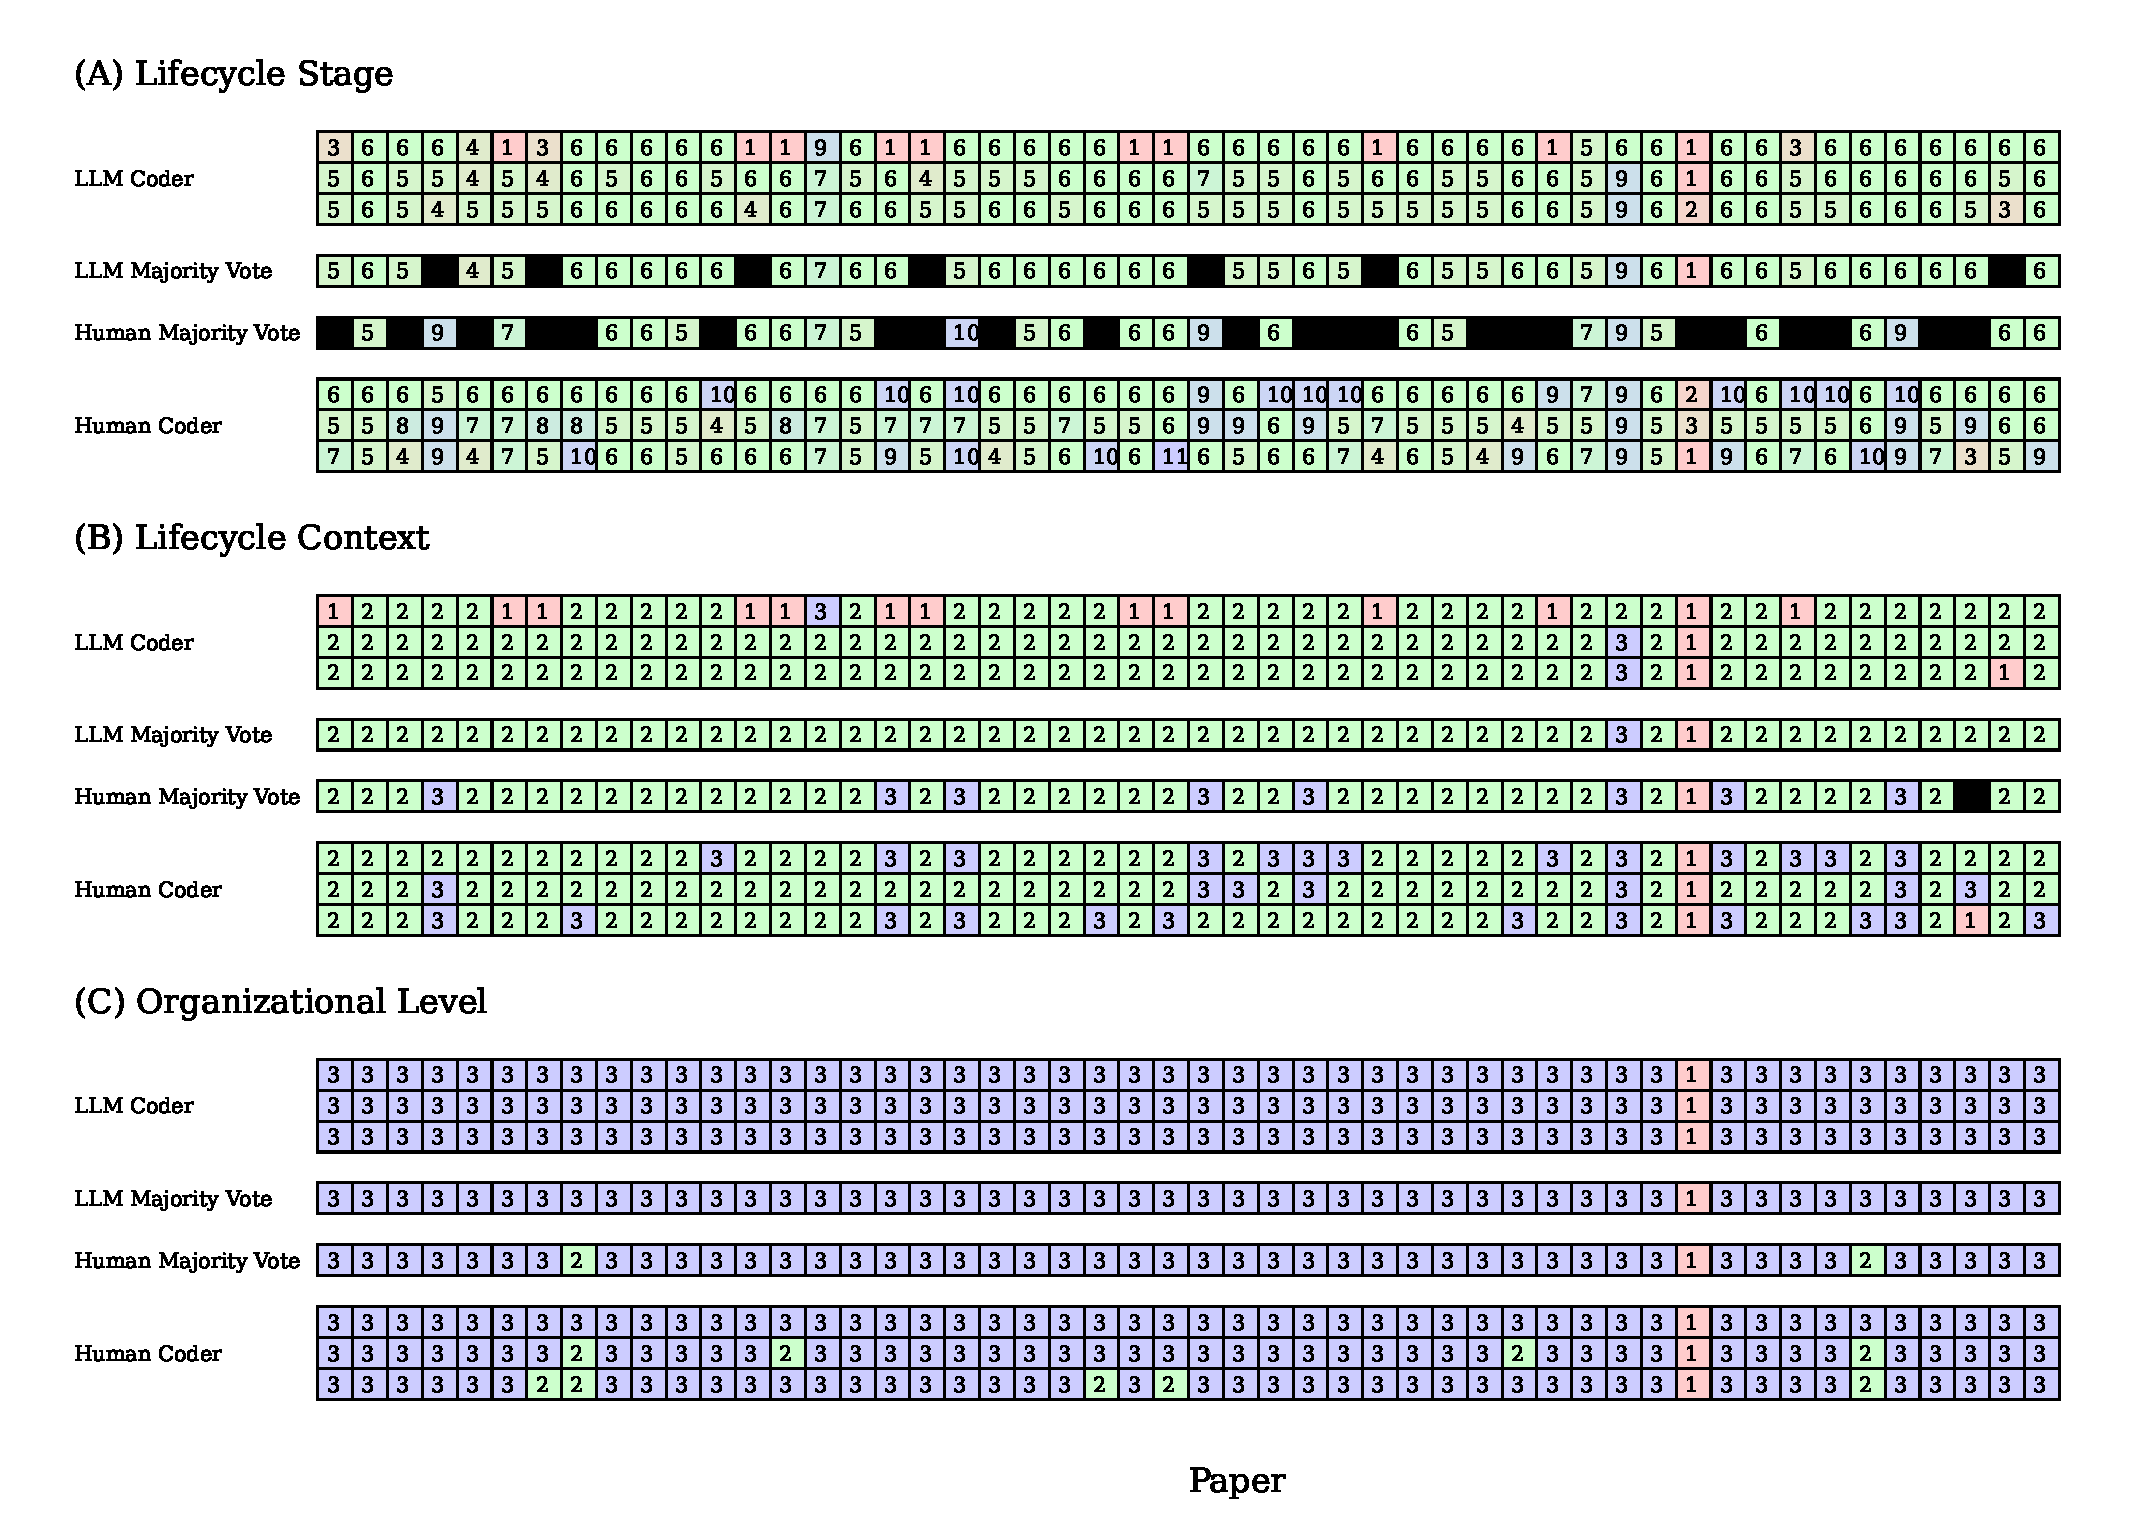
\includegraphics[width=\textwidth]{interrate.eps}
    \caption{Comparison of Human and LLM ratings on a random sample of 50 papers.  In each grid, columns correspond to papers and rows correspond to individual coders or majority votes across coder groups.  The number in each cell is the category rating (1-3 for level and context, 1-11 for systems engineering lifecycle stage, increasing from top to bottom or left to right in the categorization matrix).  Ratings are color-coded to aid visualization, with red, green, and blue corresponding to ratings 1, 2, and 3.  Individual lifecycle stages use the same color as their containing context but with a finer color gradient.  Black cells indicate papers with no clear majority vote (each coder gave a distinct rating).}
    \label{fig:interrate}
\end{figure}

\textbf{Key Takeaways:}  Our first observation is that the LLM coder group has greater internal consistency than the human coder groups, across almost all metrics and matrix axes.  This does not necessarily mean that the LLM ratings accurately reflect the paper content, but only that the LLMs have similar behavior.

Our second observation is that in almost all conditions, Krippendorff's $\alpha$ is well below 0.8, a typical threshold for reliability used in the reserch papers.  However, the IRR paper has also found that Krippendorff's $\alpha$ gives counterintuitive or paradoxical results when the rating distributions are highly skewed \cite{feinstein1990high,geijer2025some}.  This is the case in our data, since almost all papers were rated as system level (3) and solution context (2).  For example, it is clear in Figure \ref{fig:interrate}(c) that human ratings of organizational level are in high agreement, even though the corresponding Krippendorff's $\alpha$ in Table \ref{tab:inter-rataer} (bottom row, fourth column) is only 0.38.  Hence we focus on the other metrics for gauging rater reliability.

Our third observation is that ratings of systems engineering lifecycle stage are not consistent, within or across coder groups.  One explanation for this is that most papers address \textit{multiple} stages, such as system design (paper methodology), analysis (paper theoretical results), and validation (paper experimental results).  However, at the coarser resolution of lifecycle \textit{context}, there is substantially more consistency between ratings.  And organizational level ratings are highly consistent by all metrics, within and across coder groups.

Finally, and most importantly, we see that majority votes of each coder group (human and LLM) are in strong agreement, except for lifecycle stage.  This is apparent in Figure \ref{fig:interrate} and we quantify it here: For organizational level (Figure \ref{fig:interrate}(c)), the LLM majority vote matches the human majority vote in 48 of 50 papers (96\%), and for lifecycle context (Figure \ref{fig:interrate}(b)), they match in 42 of 50 papers (84\%).  This strongly suggests that, to first order, the LLM categorizations across the full $\sim 9$K paper set accurately reflect real research trends.

% We compute Krippendorff's alpha coefficients to quantify agreement between categorization approaches:

% \begin{itemize}
%     \item \textbf{Human vs. LLM Model 1}: $\alpha$ = [To be computed]
%     \item \textbf{Human vs. LLM Model 2}: $\alpha$ = [To be computed]
%     \item \textbf{Human vs. LLM Model 3}: $\alpha$ = [To be computed]
%     \item \textbf{Among Three LLMs}: $\alpha$ = [To be computed]
% \end{itemize}

% Our target threshold of $\alpha \geq 0.800$ indicates acceptable reliability for using LLM-assisted categorization while maintaining human oversight for uncertain cases.

% [Note: Actual Krippendorff's alpha values, confusion matrices, and detailed statistical analysis will be computed once all categorization results are finalized and will be inserted here.]

\begin{table}[!htbp]
\centering
\caption{Inter-Rater Reliability Metrics.}
\label{tab:interrate}
\begin{tabular}{|l|ccc|ccc|ccc|}
\toprule
Axis &  \multicolumn{3}{c}{\% Agreement} & \multicolumn{3}{c}{Krippendorff's $\alpha$} & \multicolumn{3}{c|}{Gwet's AC1} \\
\midrule
& Humans & LLMs & Both & Humans & LLMs & Both & Humans & LLMs & Both \\
Lifecycle & 0.02 & 0.30 & 0.00 & -0.02 & 0.17 & 0.07 & 0.12 & 0.44 & 0.27 \\
Context & 0.60 & 0.70 & 0.36 & 0.28 & 0.12 & 0.15 & 0.66 & 0.77 & 0.68 \\
Level & 0.86 & 1.00 & 0.86 & 0.38 & 1.00 & 0.43 & 0.90 & 1.00 & 0.94 \\
% Fine & 0.02 & 0.30 & 0.00 & -0.01 & 0.18 & 0.07 & 0.14 & 0.44 & 0.29 \\
% Coarse & 0.56 & 0.70 & 0.36 & 0.27 & 0.13 & 0.15 & 0.65 & 0.78 & 0.68 \\

\bottomrule
\end{tabular}\label{tab:inter-rataer}
\end{table}